\chapter[SCP-153 下水道蠕虫]{
    SCP-153 Drain Worms\\
    SCP-153 下水道蠕虫
}

\label{chap:SCP-153}

\begin{figure}[H]
    \centering
    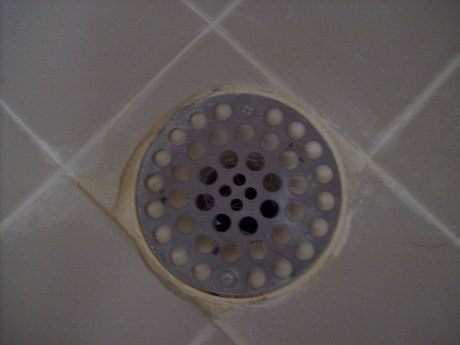
\includegraphics[width=0.5\linewidth]{images/SCP.153.jpg}
    \caption*{SCP-153一个已伪装的样本}
\end{figure}

\bb{项目编号:}SCP-153

\bb{项目等级:}Euclid

\bb{特殊收容措施:}SCP-153的样本们应该放置生物研究12区之中的一种耐酸,且尺寸不小于10米×10米×5米的容器中进行隔离饲养,并需要在容器内部区域放置一些污水和有机材料。每隔四个小时必须对容器内的有机物含量水平和结构完整性进行一次检测。绝对不允许让这些容器连接到任何内部或外部的管道。

可以肯定的是,仍然有数量不明的SCP-153样本存在于野外。任何关于人们在淋浴间和浴缸神秘失踪的报告都必须立即展开调查。探员必须配备红外线和紫外线传感器以防止被SCP-153的伪装骗过。如果可能的话,应保持样本的存活并将其移送到12区。

\bb{描述:}SCP-153最初作为一个线虫(蛔虫)的品种被发现,可达到██米的长度和██cm的直径。SCP-153的样本生活在下水道和排水管,而且可以存活于大多数的有机材料之中,它们更喜欢以动物的组织为食。

SCP-153的样本可以从它们的口和齿槽中释放一种类似于{[}数据删除]的强酸物质,并且不管是处于生物体内还是体外时都拥有伪装的能力。SCP-153已经进化出了一种捕食技巧,它们在淋浴喷头或浴缸排水孔里面游动,用它们的酸性唾液溶解排水盖,并伪装它们的食道使其看起来象是一个标准的排水孔。不久之后,人类进入淋浴间或是浴缸的时候,样本{[}数据删除],并几乎不留下任何痕迹地返回排水孔里。整个过程通常需要不到█████秒。

\bb{附录153-01:}SCP-153的样本必须保持相互隔离除非其养殖条件受到控制下。——Kovalanskaya博士

\bb{附录153-02:}事故█████████████表明SCP-153的样本通过下水道口,厕所和{[}数据删除]来展开对人们的攻击,研究人员正在调查为何一个看似如此简单的动物能够演化出这种相对复杂的捕猎技巧。

\bb{附录153-03:}Kovalanskaya博士已经得到许可,开始一次以基因工程为中心的对SCP-153的育种研究计划,该计划{[}数据删除],并被当作一个潜在的处理有机废物的方法。
